%
%	Begrifflichkeiten
%

\pagebreak
\section{NIS2}

\onehalfspacing

\subsection{The Network and Information Security Directive}

The European Commission and the High Representative of the Union for Foreign Affairs and Security Policy presented a new EU Cybersecurity Strategy at the end of 2020.\footnote{See \textit{EU (2023)}: Cybersecurity Policies. \cite{cyberPol}}

\subsubsection{Cybersecurity across the Union}

\subsubsection{The EU cybersecurity agency ENISA}

\subsubsection{Cyber Resilience Act}

\subsubsection{Cybersecurity Act}

\subsubsection{Cyber Solidarity Act}

\subsubsection{Certification}

\subsection{Center for Internet Security}

\subsubsection{CIS Controls}

\subsubsection{CIS Benchmarks}

\subsection{Rancher}

\begin{figure}[H]
\centering
\caption {Rancher Dashboard}
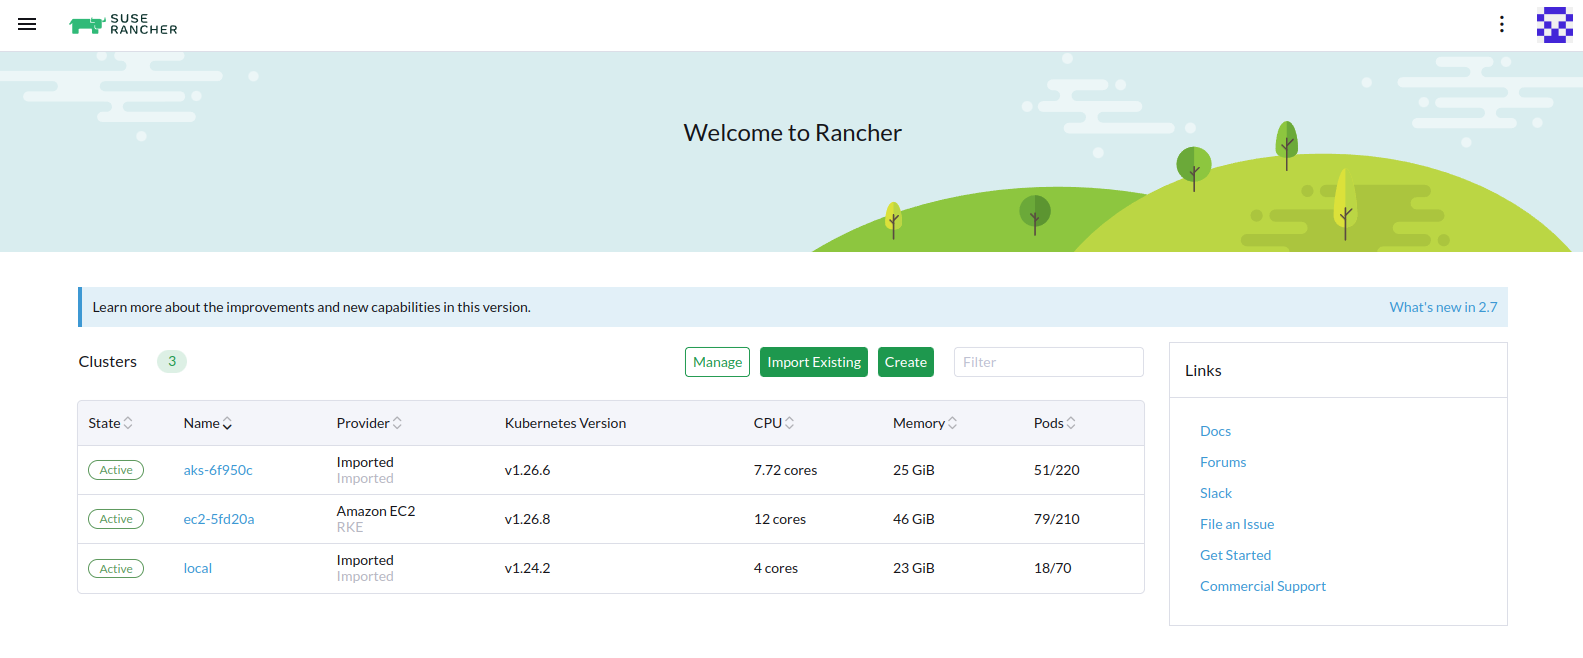
\includegraphics[width=\linewidth]{images/rancher-dashboard.png}
\label{fig:rancherDashboard}
\end{figure}

\subsubsection{CIS Benchmarks}

\subsubsection{CIS Benchmarks Installation}

\begin{lstlisting}[caption=Installing CIS Benchmarks, frame=single, basicstyle=\ttfamily]
# CIS Benchmarks
resource "rancher2_app_v2" "cisbench_fom" {
  lifecycle {
    ignore_changes = all
  }
  cluster_id = rancher2_cluster.cluster_fom.id
  name = "rancher-cis-benchmark"
  namespace = "cis-operator-system"
  project_id = data.rancher2_project.system.id
  repo_name = "rancher-charts"
  chart_name = "rancher-cis-benchmark"
  chart_version = var.cischart
}
\end{lstlisting}

\subsubsection{CIS Benchmark Reports}

\begin{itemize}
 \item AKS 1.0
 \item Kubernetes 1.6
\end{itemize}

\subsection{Methodology}
